\begin{surferPage}{Ein Doppelkegel}
    Wie in der Einleitung zu dieser Galerie erklärt, heißt eine Fläche
    \emph{nicht-singulär}, 
    wenn sie, anschaulich gesagt, 
    keine spitzen Stellen, Singularitäten genannt, hat, z.B.\ eine Kugel, 
    ein Torus (1.\ bzw.\ 2.\ Bild von links):
    \begin{center}
      \begin{tabular}{@{}c@{}c@{}c@{}c@{}}
        \begin{tabular}{@{}c}
          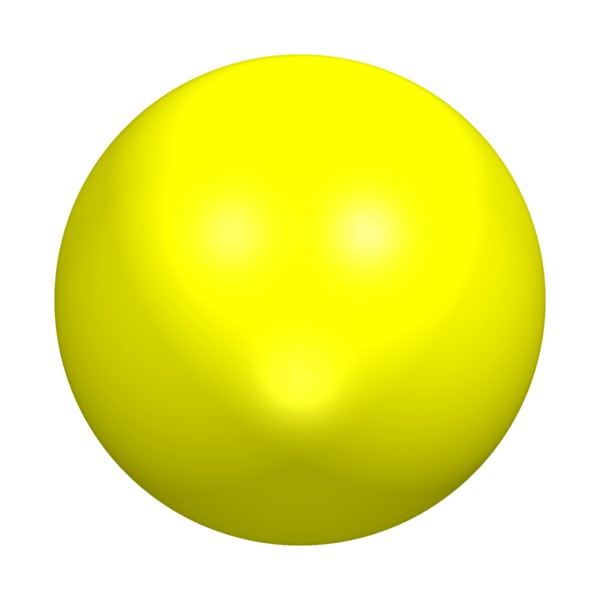
\includegraphics[width=1.4cm]{./../../common/images/kugel}
        \end{tabular}
        &
        \begin{tabular}{@{}c}
          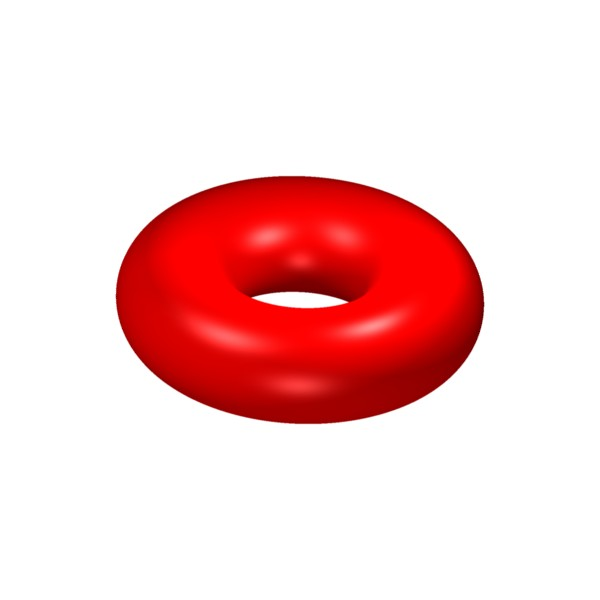
\includegraphics[width=1.4cm]{./../../common/images/torus}
        \end{tabular}
        &
        \begin{tabular}{c@{}}
          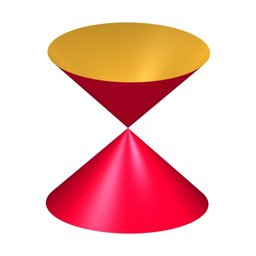
\includegraphics[width=1.4cm]{./../../common/images/kegel}
        \end{tabular}
      \end{tabular}
    \end{center}
    Der Doppelkegel (rechtes Bild) ist die einfachste Singularität; 
    er ist z.B.\ die einzige, die man schon durch eine
    Gleichung vom Grad $2$ beschreiben kann:
    \[x^2+y^2-z^2=0.\]
    Ändert man diese leicht, indem man auf der rechten Seite der
    Gleichung einen Wert $a\neq 0$ hinschreibt, so verwandelt er sich, je
    nach Vorzeichen von $a$, in einen der Hyperboloiden: 
    \begin{center}
      \begin{tabular}{@{}c@{\ }c@{\ }c@{\ }c@{\ }c@{}}
        \begin{tabular}{@{}c@{}}
          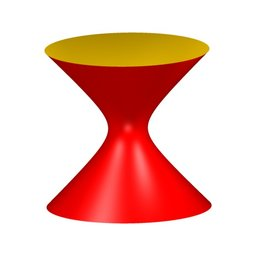
\includegraphics[width=1.2cm]{./../../common/images/A1pm_2}
        \end{tabular}
        &
        $\leftarrow$
        &
        \begin{tabular}{@{}c@{}}
          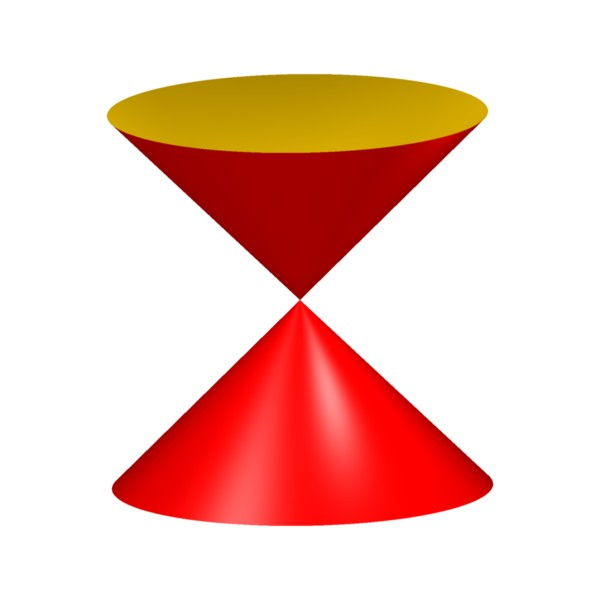
\includegraphics[width=1.2cm]{./../../common/images/A1pm_1} 
        \end{tabular}
        &
        $\rightarrow$
        &
        \begin{tabular}{@{}c@{}}
          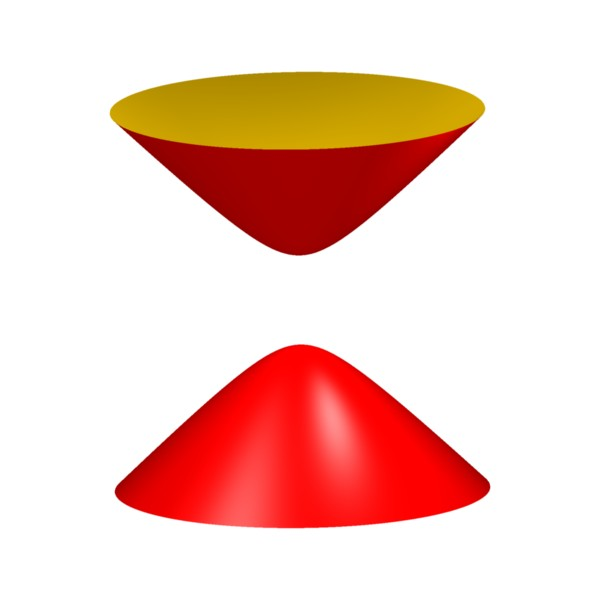
\includegraphics[width=1.2cm]{./../../common/images/A1pm_0}
        \end{tabular}
      \end{tabular}
    \end{center}
    Eine Fläche vom Grad $2$ hat höchstens eine Singularität, 
    d.h.\ $\mu(2)=1$.
\end{surferPage}
